\documentclass{article}
\usepackage{amsmath}
\usepackage[pdftex]{graphicx}
\usepackage{subfigure}
\usepackage{indentfirst}

\title{Information Theoretic Modeling -- Exercise 5}
%\author{Haibo Jin}
\date{}


\bibliographystyle{plain}

\begin{document}

\maketitle

{\centering \large \textbf{Haibo Jin}}

{\centering \large \textbf{Student number: 014343698}}

\section{Problem 1}

Please refer to \emph{$markov\_chain.py$} code for more details.

\subsection*{(a)}

The probability of the data given a parameter $\theta$ is:

\vspace{2mm}

$p(D)=\int_{\Theta}p_{\theta}(D)d_{\theta}=\int_{\Theta}\theta^k(1-\theta)^{n-k}d_\theta$

\vspace{2mm}

Since the prior is $B(0.5,0.5)$, so the $\theta$ is uniformly distributed. Under mixture code with zero-order, then the average probability is just the probability of a point in beta-binomial distribution:

\vspace{2mm}

$pmf=\frac{B(k+\alpha, n-k+\beta)}{B(\alpha, \beta)}$

\vspace{2mm}

I implemented a program to get the count of 1 and 0, then calculate the probability: $p=9.27\times10^{-26}$. Then the code-length is: $-log_2p=83.156$

\subsection*{(b)}

Since it is first-order model, there are two parameters:

\vspace{2mm}

$\theta_0=p(x_i=1|x_{i-1}=0)$ and $\theta_1=p(x_i=1|x_{i-1}=1)$

\vspace{2mm}

Then the original data can be divided into three parts:

\vspace{2mm}

$p(D)=p(D_1) \times p(D_2) \times p(D_3)$

\vspace{1mm}

$=p(x_1=1)\times\int{\theta_0}^{k_0}(1-\theta_0)^{n-k_0}d_{\theta_0}\times\int{\theta_1}^{k_1}(1-\theta_1)^{n-k_1}d_{\theta_1}$

\vspace{2mm}

That is to say, the mixture code with first-order can be computed with multiplying the probability of the first symbol, the probability of a zero-order model in which symbols occur after 0, and the probability of a zero-order model in which symbols occur after 1.

\vspace{2mm}

Based on the running result of the program, $p=1.18 \times 10^{-26}$. Then the code-length is: $-log_2p=86.128$

\subsection*{(c)}

Similar as the first-order model, the second-order model just divide the original into five parts, one of which is the probability of the first two symbols and another four zero-order models. The result is $p=8.67 \times 10^{-28}$ and code-length is $-log_2p=89.896$

\section{Problem 2}

Problem 2 is also implemented in \emph{$markov\_chain.py$}, please see it for more details.

\subsection*{(a)}

Using NML model, the probability of the data with zero-order is $p=8.83 \times 10^{-26}$. The code-length is $-log_2p=83.227$. 

\subsection*{(b)}

Using NML model, the probability of the data with zero-order is $p=1.01 \times 10^{-26}$. The code-length is $-log_2p=86.346$. 

\subsection*{(c)}

Using NML model, the probability of the data with zero-order is $p=5.67 \times 10^{-28}$. The code-length is $-log_2p=90.51$. 

\section{Problem 3 and 4}

Firstly, I just tried several functions:
\vspace{2mm}

Functions with $k=2$ (including $\sigma$):

\vspace{1mm}

$f(x)=ax^2$ and the RSS=1623.11

\vspace{1mm}

$f(x)=ax^3$ and the RSS=3990.66

\vspace{1mm}

Functions with $k=3$ (including $\sigma$):

$f(x)=a+bx^2$ and the RSS=1375.7

\vspace{1mm}

$f(x)=a+bx^3$ and the RSS=1844.83

\vspace{1mm}

$f(x)=ax+bx^2$ and the RSS=1472.92

\vspace{1mm}

$f(x)=ax^b$ and the RSS=1521.48

\vspace{1mm}

Functions with $k=4$ (including $\sigma$):

$f(x)=a+bx+cx^2$ and the RSS=1367.67

\vspace{1mm}

$f(x)=a+bx+csin(x)$ and the RSS=1368.83

\vspace{1mm}

$f(x)=a+bx+ccos(x)$ and the RSS=1563.27

\vspace{1mm}

Functions with $k=5$ (including $\sigma$):

$f(x)=a+bx+cx^2+dx^3$ and the RSS=1357.02

\vspace{1mm}

After observing the above examples and their RSS values, I found that some formulas are just better than other formulas for this data. For example, with $k=2$, $f(x)=ax^2$ is just a good approximation; with $k=3$, $f(x)=a+bx^2$ and $f(x)=ax+bx^2$ are both good.

Since this final code-length just consists of two parts: the length of parameters and length of data, we of course want to choose those functions with less parameters but less RSS value. And this is just a trade-off between model complexity and its performance. If I want to get a better approximation, maybe I should reuse those good functions in their corresponding groups (i.e. the value of k). Some functions with less parameter may perform well, but not optimal. If we can combine those good functions, we may get less RSS value and maybe also offset the increase because of parameters. Then I tried these functions based on my previous attempts:

Functions with $k=4$ (including $\sigma$):

\vspace{1mm}

$f(x)=a+bx^2+csin(x)$ and the RSS=1366.82, code-length=1056.94

\vspace{5mm}
\begin{minipage}{0.9\textwidth}
  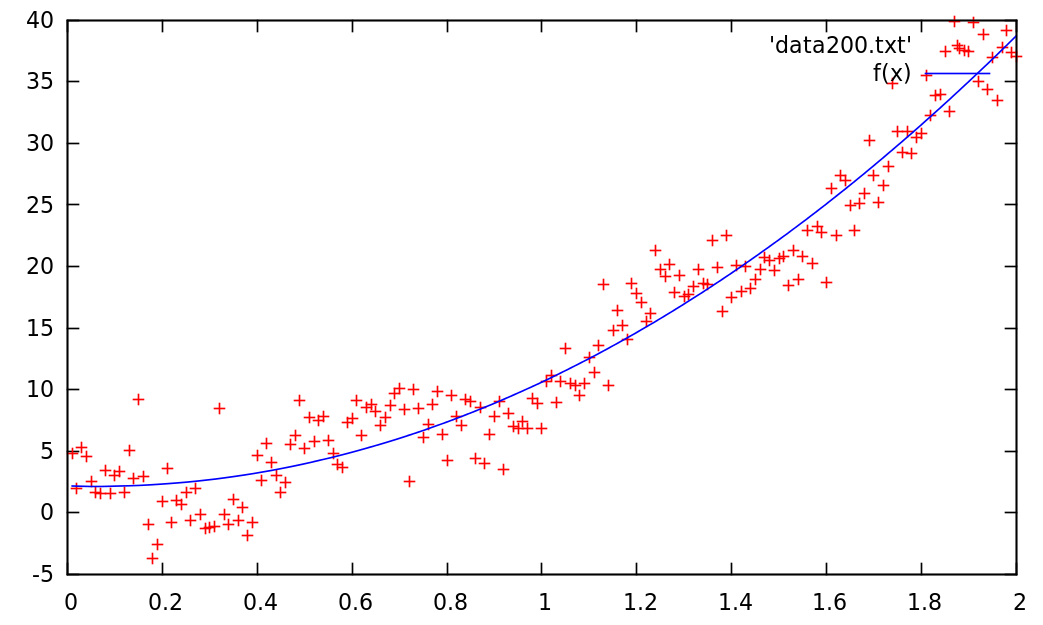
\includegraphics[width=\textwidth,keepaspectratio]{19.png}
  \centerline{Figure 1: Fit plot of $f(x)=a+bx^2+csin(x)$}
\end{minipage}
\vspace{5mm}

$f(x)=ax^b+cx^2$ and the RSS=1357.94, code-length=1056.008

\vspace{5mm}
\begin{minipage}{0.9\textwidth}
  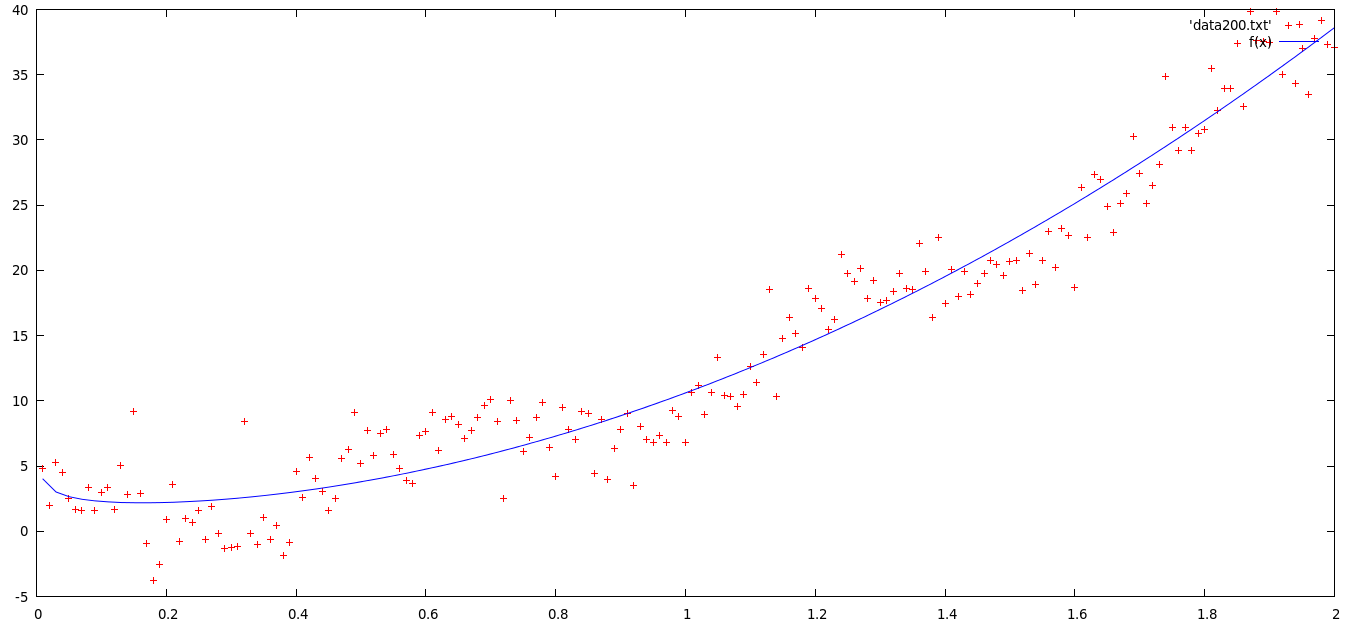
\includegraphics[width=\textwidth,keepaspectratio]{22.png}
  \centerline{Figure 2: Fit plot of $f(x)=ax^b+cx^2$}
\end{minipage}
\vspace{5mm}

Functions with $k=5$ (including $\sigma$):

\vspace{1mm}

$f(x)=a+bx^2+csin(dx)$ and the RSS=1366.71, code-length=1060.75

\vspace{5mm}
\begin{minipage}{0.9\textwidth}
  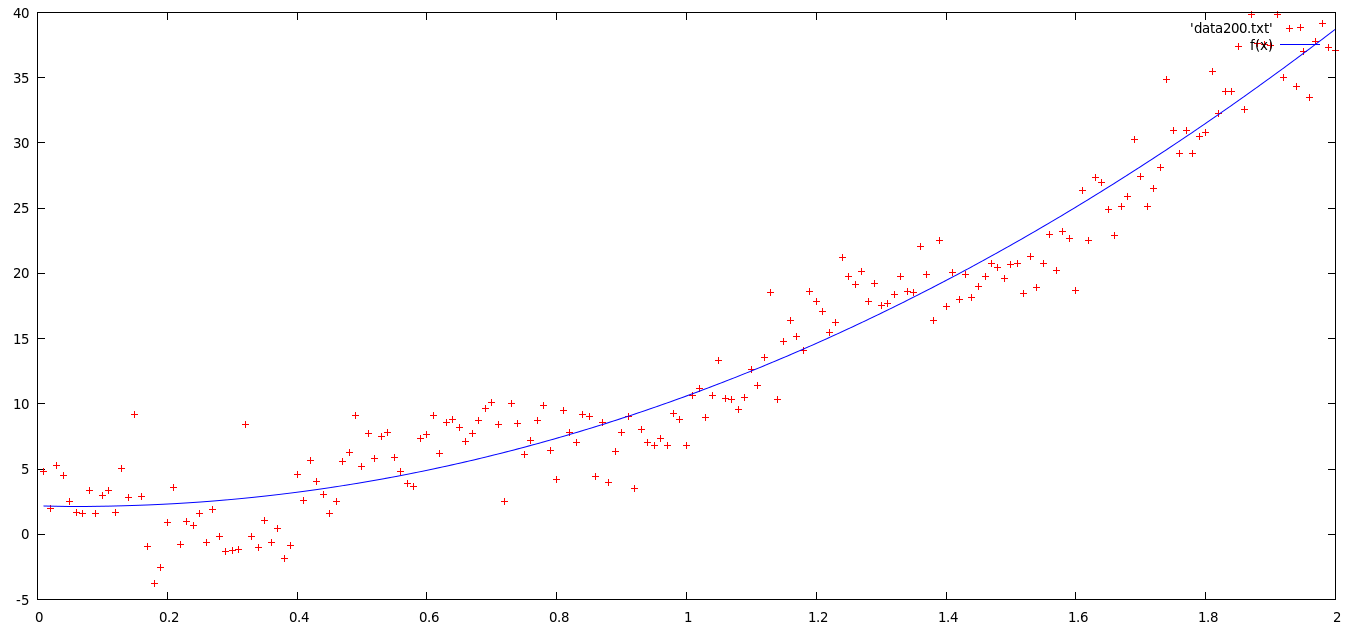
\includegraphics[width=\textwidth,keepaspectratio]{20.png}
  \centerline{Figure 3: Fit plot of $f(x)=a+bx^2+csin(dx)$}
\end{minipage}
\vspace{5mm}

\vspace{1mm}

$f(x)=ax^b+cx^2+dsin(x)$ and the RSS=1356.95, code-length=1059.72

\vspace{5mm}
\begin{minipage}{0.9\textwidth}
  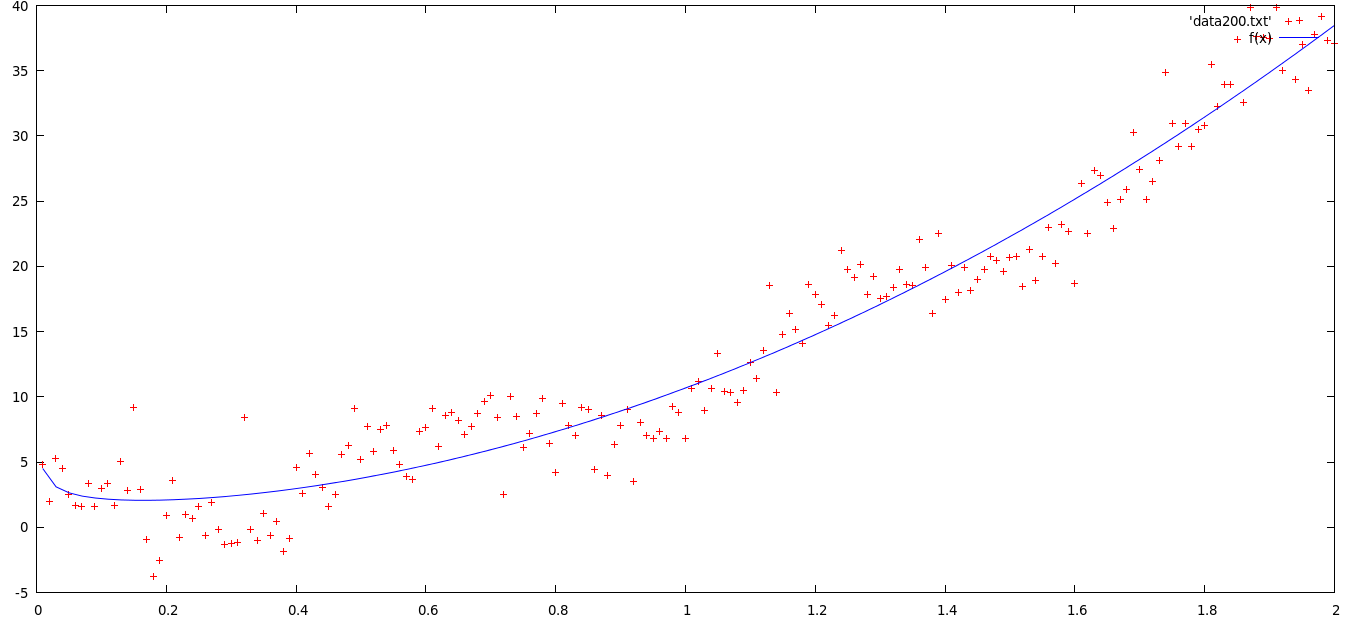
\includegraphics[width=\textwidth,keepaspectratio]{23.png}
  \centerline{Figure 4: Fit plot of $f(x)=ax^b+cx^2+dsin(x)$}
\end{minipage}
\vspace{5mm}

\vspace{1mm}

Following this thought, the performance do become better. And the best function I found is $f(x)=ax^b+cx^2$, and its final length-code is 1056.008 

\end{document}